% Rebuild: xelatex -no-pdf -interaction=nonstopmode finger-tree-1.tex
%          dvisvgm --no-fonts --exact-bbox finger-tree-1.xdv -o finger-tree-1.svg
\def\pgfsysdriver{pgfsys-dvisvgm.def}
\documentclass[tikz,border=4pt]{standalone}
\usetikzlibrary{arrows.meta,backgrounds}
\begin{document}
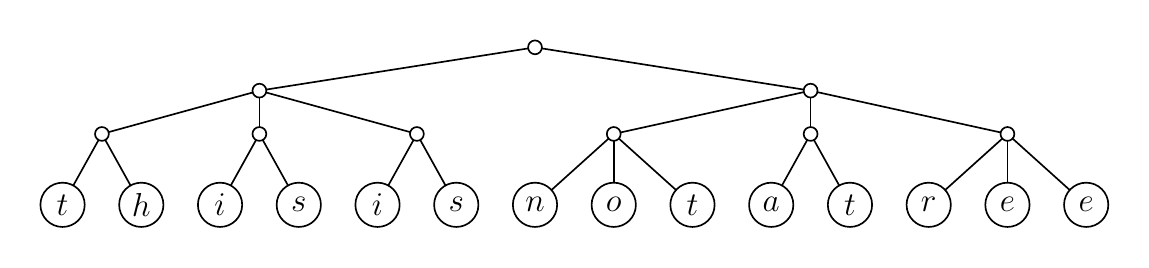
\begin{tikzpicture}[background rectangle/.style={fill=white},show background rectangle,x=1cm,y=1cm,line width=.6pt,
  internal/.style={circle,draw,fill=white,inner sep=0pt,minimum size=5pt},
  leaf/.style={circle,draw,fill=white,inner sep=0pt,minimum size=16pt,font=\large}]
\coordinate (root) at (6,2);
\coordinate (left) at (2.5,1.45);
\coordinate (right) at (9.5,1.45);
\coordinate (g0) at (0.5,0.9);
\coordinate (g1) at (2.5,0.9);
\coordinate (g2) at (4.5,0.9);
\coordinate (g3) at (7,0.9);
\coordinate (g4) at (9.5,0.9);
\coordinate (g5) at (12,0.9);
\coordinate (l0) at (0,0);
\coordinate (l1) at (1,0);
\coordinate (l2) at (2,0);
\coordinate (l3) at (3,0);
\coordinate (l4) at (4,0);
\coordinate (l5) at (5,0);
\coordinate (l6) at (6,0);
\coordinate (l7) at (7,0);
\coordinate (l8) at (8,0);
\coordinate (l9) at (9,0);
\coordinate (l10) at (10,0);
\coordinate (l11) at (11,0);
\coordinate (l12) at (12,0);
\coordinate (l13) at (13,0);
\draw (root) -- (left);
\draw (root) -- (right);
\draw (left) -- (g0);
\draw (left) -- (g1);
\draw (left) -- (g2);
\draw (right) -- (g3);
\draw (right) -- (g4);
\draw (right) -- (g5);
\draw (g0) -- (l0);
\draw (g0) -- (l1);
\draw (g1) -- (l2);
\draw (g1) -- (l3);
\draw (g2) -- (l4);
\draw (g2) -- (l5);
\draw (g3) -- (l6);
\draw (g3) -- (l7);
\draw (g3) -- (l8);
\draw (g4) -- (l9);
\draw (g4) -- (l10);
\draw (g5) -- (l11);
\draw (g5) -- (l12);
\draw (g5) -- (l13);
\node[internal] at (root) {};
\node[internal] at (left) {};
\node[internal] at (right) {};
\node[internal] at (g0) {};
\node[internal] at (g1) {};
\node[internal] at (g2) {};
\node[internal] at (g3) {};
\node[internal] at (g4) {};
\node[internal] at (g5) {};
\node[leaf] at (l0) {$t$};
\node[leaf] at (l1) {$h$};
\node[leaf] at (l2) {$i$};
\node[leaf] at (l3) {$s$};
\node[leaf] at (l4) {$i$};
\node[leaf] at (l5) {$s$};
\node[leaf] at (l6) {$n$};
\node[leaf] at (l7) {$o$};
\node[leaf] at (l8) {$t$};
\node[leaf] at (l9) {$a$};
\node[leaf] at (l10) {$t$};
\node[leaf] at (l11) {$r$};
\node[leaf] at (l12) {$e$};
\node[leaf] at (l13) {$e$};
\end{tikzpicture}
\end{document}
